\documentclass[UTF8]{ctexart}
\usepackage{amsmath}
\usepackage{mathtools}
\usepackage{geometry}
\usepackage{tikz}
\usepackage{enumitem}
\usepackage{ulem}
\setitemize{topsep=-0.3cm}
\geometry{a4paper,scale=0.77}
\title{每日一题(4.2)答案}
\author{选题:李衡岳,程昊一\\答案制作:程昊一}
\begin{document}
\maketitle
\begin{itemize}
\item[\textbf{1.}]{\CJKfamily{kai}用含$n$的代数式表示$1^4+2^4+\dots+n^4$,其中$n$为正整数.\\
(程昊一供题)}\\
\hspace*{2em}\textbf{解}\quad 我们知道,$\sum\limits_{i=1}^{n}i^2=\dfrac{n(n+1)(2n+1)}{6}$.\\其中$\sum$的用法参见\uline{https://baike.baidu.com/item/∑/1233796}.\\
\hspace*{2em}我们现在来思考$\sum\limits_{i=1}^{n}i^3$.\\
\hspace*{2em}注意到\[\sum\limits_{i=1}^{n}i(i+1)(i+2)=\dfrac{n(n+1)(n+2)(n+3)}{4}\]
而且对于每一个$i(i=1,2,\dots ,n)$,我们都有
\[i^3=i(i+1)(i+2)-3i^2-2i\]
所以,
\begin{align*}
&\sum\limits_{i=1}^{n}i^3\\
=&\sum\limits_{i=1}^{n}(i(i+1)(i+2)-3i^2-2i)\\
=&\sum\limits_{i=1}^{n}i(i+1)(i+2)-3\sum\limits_{i=1}^{n}i^2-2\sum\limits_{i=1}^{n}i\\
=&\frac{n(n+1)(n+2)(n+3)}{4}-\frac{n(n+1)(2n+1)}{2}-n(n+1)\\
=&\frac{n(n+1)(n+2)(n+3)-2n(n+1)(2n+1)-4n(n+1)}{4}\\
=&\frac{n(n+1)[(n+2)(n+3)-2(2n+1)-4]}{4}\\
=&\frac{n(n+1)(n^2+n)}{4}\\
=&\frac{n^2(n+1)^2}{4}
\end{align*}
\hspace*{2em}我们再来看$\sum\limits_{i=1}^{n}i^4$.\\
\hspace*{2em}注意到\[\sum\limits_{i=1}^{n}i(i+1)(i+2)(i+3)=\frac{n(n+1)(n+2)(n+3)(n+4)}{5}\]
而且对于每一个$i(i=1,2,\dots,n)$,我们都有
\[i^4=i(i+1)(i+2)(i+3)-6i^3-11i^2-6i\]
所以,
\begin{align*}
&\sum\limits_{i=1}^{n}i^4\\
=&\sum\limits_{i=1}^{n}(i(i+1)(i+2)(i+3)-6i^3-11i^2-6i)\\
=&\sum\limits_{i=1}^{n}i(i+1)(i+2)(i+3)-6\sum\limits_{i=1}^{n}i^3-11\sum\limits_{i=1}^{n}i^2-6\sum\limits_{i=1}^{n}i\\
=&\frac{n(n+1)(n+2)(n+3)(n+4)}{5}-\frac{3n^2(n+1)^2}{2}-\frac{11n(n+1)(2n+1)}{6}-3n(n+1)\\
=&\frac{6n(n+1)(n+2)(n+3)(n+4)-45n^2(n+1)^2-55n(n+1)(2n+1)-90n(n+1)}{30}\\
=&\frac{n(n+1)[6(n+2)(n+3)(n+4)-45n(n+1)-55(2n+1)-90]}{30}\\
=&\frac{n(n+1)(6n^3+9n^2+n-1)}{30}\\
=&\frac{n(n+1)(2n+1)(3n^2+3n-1)}{30}
\end{align*}
\hspace*{2em}所以,$\sum\limits_{i=1}^{n}i^4=\dfrac{n(n+1)(2n+1)(3n^3+3n-1)}{30}$.
\item[\textbf{2.}]{\CJKfamily{kai}平面上有25个点,任意三点之中必然存在两个点,它们的距离小于1.证明:必然能找到13个点,它们位于半径为1的圆中.\\
(程昊一供题)}\\
\hspace*{2em}\textbf{分析}\quad 我们要搞清楚“任意三点中必然存在两点,它们的距离小于1”这个条件意味着什么,还要搞清楚“13个点位于半径为1的圆中”意味着什么.\\
\hspace*{2em}\textbf{解}\quad 我们任选一个点$A$,将其余24个点做如下\textbf{分类}:将与$A$的距离小于1的点分为第一类$S_1$,将与$A$的距离大于等于1的点分为第二类$S_2$.我们用$|S_1|$表示$S_1$中点的个数,$S_2$同理.\\
\begin{figure}[!ht]
\centering
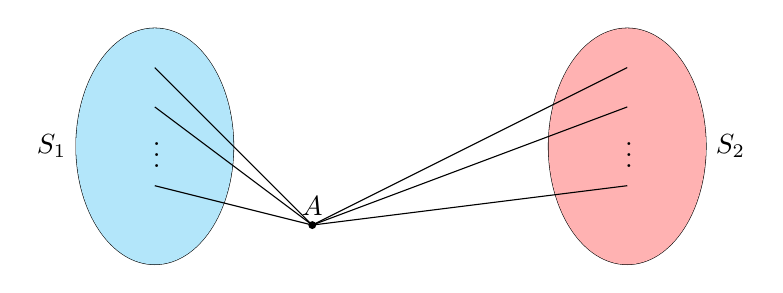
\begin{tikzpicture}
	\node at (0,0)[above]{$A$};
	\fill (0,0) circle(0.05);
	\draw (-2,1) ellipse(1 and 1.5);
	\fill (-2,1) [color=cyan!30] ellipse(1 and 1.5);
	\draw (0,0)--(-2,1.5);
	\draw (0,0)--(-2,0.5);
	\draw (0,0)--(-2,2);
	\node at (-3,1)[left]{$S_1$};
	\node at (-2.15,1)[right]{$\vdots$};
	\draw (4,1) ellipse(1 and 1.5);
	\fill (4,1) [color=red!30] ellipse(1 and 1.5);
	\draw (0,0)--(4,2);
	\draw (0,0)--(4,1.5);
	\draw (0,0)--(4,0.5);
	\node at (5,1)[right]{$S_2$};
	\node at (3.85,1)[right]{$\vdots$};
\end{tikzpicture}
\end{figure}

\hspace*{2em}若$|S_1|\ge12$,则我们以$A$为圆心,1为半径作圆,因为对于任意一点在$S_1$中的$P$,都有$AP\le1$,所以$A$和$S_1$中的点都在此圆中,命题得证.\\
\hspace*{2em}若$|S_1|<12$,因为$|S_1|+|S_2|=24$,所以$|S_2|\ge13$.此时任取$S_2$中的一个点$Q$.对于$S_2$中的其余任意一点$T$,因为任意三点中存在两点的距离小于1,所以$AQ,AT,QT$中必然有一个小于1.又$AQ\ge1,AT\ge1$,所以$QT<1$.也就是说,对于$S_2$中其余任何一点,都有$Q$与这个点的距离小于1.则$S_2$中的其余任何点都在以$Q$为圆心,1为半径的圆中,即$S_2$中的任何点都在此圆中,命题得证.\\
\hspace*{2em}综上:原命题得证.


\end{itemize}
\end{document}